\section{Diskussion}
\label{sec:diskussion}
%Detta avsnitt innehåller en sammanfattning av konstruktionen och en diskussion av resultatet. Om det
%är möjligt, dra slutsatser av ert projekt och identifiera förbättringsmöjligheter
%(vilka kan vara användbara för en beställare).
Slutresultatet uppnår de krav som sattes på arbetet, se \ref{sec:kravspec}. Larmenheten, dörrenheten och centralenheten arbetar tillsammans för att uppfylla de krav som ställdes för ett fungerande lås- och larmsystem. Centralenheten övervakar enheternas status regelbundet. Vid otillåtet intrång skickar dörrlarmet respektive rörelselarmet en signal att larma. Kommunikationen mellan enheterna sker på ett konsekvent sätt med det designade CAN-protokollet. Centralenheten lägger till enheter på ett modulärt sätt, enligt krav åtta. Däremot är det inte perfekt då ID-nummer inte delas ut dynamiskt utan är hårdkodade hos enheterna. Trots detta är systemet på bra väg att vara modulärt.
\newline \newline
Utöver grundsystemet utfördes också två utökningar av rörelselarmet. Rörelselarmet larmar lokalt inom ett visst distansintervall från rörelesesensoren och sedan globalt då intervallet överskrids. Sedan har dessutom en distinkt larmsignal framställts.
\subsection{Struktur}
\label{sec:structfunc}
Under projektets utveckling har det lagts en viss vikt på att generalisera hanteringen av modultyperna. Denna generalisering underlättas mest av modul-structen som beskrivs i sektion \ref{sec:centralenhetDL}. Att använda en gemensam datatyp för modultyperna gör det enklare att samla alla enheters information på samma ställe, i en sorts lista. Listan med enheter skulle kunna filtreras, sorteras och sökas i, vilket är en stor fördel. Om systemet skulle utökas blir dessa funktioner praktiska, mest för användaren. 
\newline \newline 
När information om en specifik modul ska uppdateras är användingen av en lista lämplig; listan söks igenom, och enhetens modul-struct uppdateras. Detta gör det möjligt för centralenheten att lagra aktuell information om alla enheter, enligt krav två i \ref{sec:kravspec}. Att samtlig information om enheterna lagras på samma plats underlättar också för utvecklare. En ny modultyp skulle kunna läggas till i systemet utan att behöva ändra på projektets struktur.
\newline \newline
Denna struktur gör dock systemet mer komplicerat, och detta kan ha negativa effekter. En komplex struktur gör det svårare att identifiera misstag eller logiska fel. Därför kan systemets säkerhet och funktionalitet bli svårare att verifiera. Men om ett komplext systems kod är en välskriven och verifierad bas för systemet främjar detta framtida utveckling. Då underlättar den befintliga koden förståelse och vidareutveckling av systemet.
\newline \newline 
En stor förbättring när det gäller generalisering skulle vara att skapa en universell modultyp för sensorer. I det nuvarande läget har larmenheten hand om vibrationssensorn och rörelsesensorn, medan dörrenheten har hand om flera magnetkontakter (eller dörrsensorer). Om en sensormodul implementeras skulle den kunna hantera alla sensorer som tidigare var kopplade till larmenheten och dörrenheten samtidigt, och utöver det skulle den kunna hantera ännu fler sensortyper. Modulens datahantering kan implementeras som centralenhetens: en generell struct för sensorer finns, och information lagras om dessa i modulens minne. Alla funktioner som är specifika för att konfigurera samt avläsa sensorerna skulle då kunna skrivas separat, och importeras av modulen som ett programbibliotek. Detta underlättar processen att lägga till en ny sensortyp.

\subsection{Funktionalitet och IO} % inte färdig
\label{sec:funktionalitet}

%Utvärdera hur enkelt det är att använda programmet, vad man kan göra. 

%USART skulle kunna skriva ut automatiska status-uppdateringar vid konfiguration ändringar och liknande. I nu-fallet om en modul konfigureras så kollas det om inmatningen fungerar, och i så fall antas att konfigureringen sker korrekt. Istället skulle funktionerna kunna skriva ut de konfigurerade enheternas nya status efter ändringen för att tydligare visa vad som har hänt. \\

%Vissa kommandon till programmet skulle kunna förtydligas och utökas. Help kommandot ger en kort beskrivning av vad varje kommando gör, vilket är korrekt. En addition skulle vara att göra det möjligt att skriva "Help [kommando]" för att ge extra information och detaljer om varje kommando. Utan detta behöver användaren ha tillgång till projektrapporten för att fullt förstå hur ett kommando fungerar.

%Diskutera användarens möjlighet att påverka systemet och systemets möjlighet att presentera information och visa resultatet av användarens påverkan.

Funktionellt skall systemet tillåta användaren att påverka systemet samt presentera information och visa resultatet av användarens påverkan. Användaren har två olika sätt att interagera med systemet: genom USART-kommandon och genom en knappsats. Detta tillåter att alla perifirienheter kan konfigureras fullständigt vilket täcker kraven på funktionalitet. \\

Systemets förmåga att ge användaren feedback är i nuläget begränsad. Centralenheten begär inte information från periferienheterna när de konfigureras. Därmed kommer ingen automatiskt utdata om ändringarnas effekt. Den lokala statusen kan fortfarande ses manuellt med USART-kommandon, men den kan vara olika från statusen på periferienheterna. Det uppnår kraven på funktionalitet, men operationen kan förenklas och optimeras. \\ 

Projektets moduler läggs nu till automatiskt vid uppstart, förutsatt att alla periferienheter har sina ID-nummer fördefienerade. Denna process är dock inte helt konfigurationsfri; användaren behöver defienera alla periferienheters ID i respektive källkod innan koden laddas. Detta skulle kunna förbättras och en utveckling av systemet är därför att implementera automatisk ID-utdelning för att göra det mer användarvänligt. Vid uppstart skulle centralenheten då dela ut ett unikt ID-nummer till alla enheter. Detta skulle göra systemet helt konfigurationsfritt och användaren skulle bara behöva koppla in de nödvändiga enheterna och trycka ''start''. 
\newline \newline 
Om den automatiska ID-utdelningen implementeras kan man anse att systemet är fullständigt modulärt. Det kan då kopplas flera dörr- och larmenheter till systemet, och det antalet moduler som kan vara kopplade samtidigt kan ändras. 
Ett icke-modulärt system, som har ett fast antal enheter, kan vara enklare att använda och det kan också vara säkrare. Att inte ha en uppstartfas som lägger till alla tillkopplade enheter minimerar risken att en oönskad modul kan läggas till i systemet, och att ändra på systemet kanske  blir svårare eftersom CAN-systemet inte skulle vara lika generellt. Den negativa sidan med ett sådant system är så klart att det inte är modulärt.

\subsection{Delsystemen}
% Nätverkslagret
Nätverkslagret tillfredsställer i slutändan projektets krav för kommunikation. Enheterna kan kommunicera genom en gemensam CAN-buss där meddelandekollisioner löses utav det skapade CAN-biblioteket. Genom prestandatester som beskrivs i \ref{sec:resultat} säkerställs, med hög sannolikhet, att nätverkslagret är robust för sabotage och tekniska fel. Däremot hade förbättringar kunnats göra som exempelvis att kryptera datan som skickas över bussen. Detta nämns mer i \ref{sec:sakerhet}. En annan förbättring hade kunnat vara att inkludera ett så kallat \textit{ACK-fält} i CAN-ramen. Det denna gör beskrivs i \ref{sec:can}. Att ha detta fält hade kunnat säkerställa att meddelanden som läggs ut på bussen faktiskt når den avsedda mottagaren. Då hade potentiellt snabbheten hos CAN-meddelandena försämrats då mer information måste utbytas. Däremot bör denna prestandaförändring vara oväsentlig.
\newline\newline
%Larmenheten
Larmenheten hanterar dess uppgifter enligt ställda krav. Avbrott prioriteras och utför ändringar omedelbart utan att påverka prestandan av sensorerna. En potentiell utökning av antalet möjliga sensorer av samma typ skulle gynna systemet i hög grad. Det skulle kräva en omstrukturering av GPIO-pinnarna samt att alla sensorfunktioner i programlogiken måste modifieras för att hantera fler än bara en modul i taget. Det skulle resultera i en drastisk minskning av antal MD407-kort för fullständiga system, med en potentiellt minimal försämring av prestanda. 
%Dörrenheten
\newline\newline
Dörrenheten är satt att hantera max åtta dörrar. Ett MD407-kort har 32 GPIO-pinnar. Varje dörr kräver tre, en för dörrsensorn och två för dioderna. Den fysiska begränsningen är alltså tio dörrar. Valet att ha max åtta dörrar gjordes med anledning av enkelhet för användaren. På MD407-kortet är pinnarna uppdelade i fyra grupper, pinnarna 0-7 och pinnarna 8-15 för både GPIOE och GPIOD, se bild \ref{fig:doorgpio}. 
Det finns alltså plats för två dörrsensorer och fyra dioder till på GPIOE 8-15. Nackdelen med det blir att användaren som skall koppla upp systemet får en mindre intuitiv och rörigare uppkoppling då en GPIO-port kommer vara både utport och inport, alltså ha både dörrsensorer och dioder. Därav valdes åtta dörrar.
\begin{figure}[h]
    \centering
    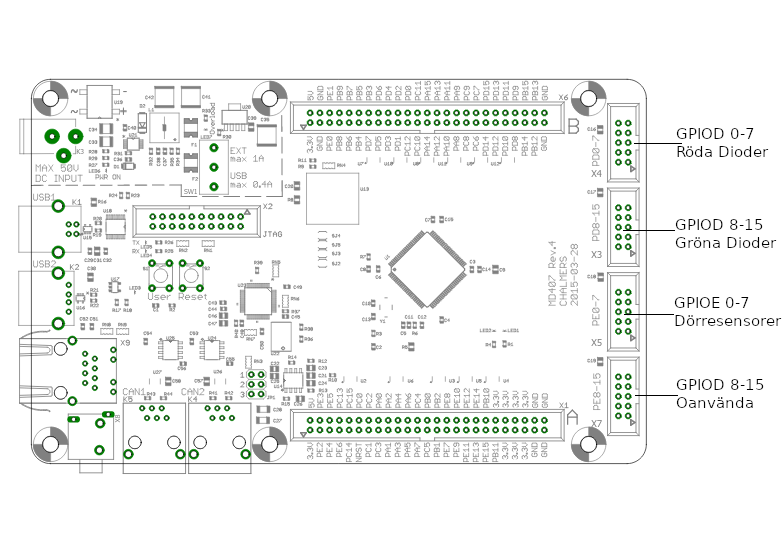
\includegraphics[scale=0.55]{dokumentation/projektrapport/IMAGES/doorgpio.png}
    \caption{GPIO-pinnarnas användning på dörrenheten\cite{md407}}
    \label{fig:doorgpio}
\end{figure}
\subsection{Säkerhet}
\label{sec:sakerhet}
Vissa åtgärder togs för att förbättra säkerheten. Alla funktioner i programmet kontrollerar sin indata innan något görs med den för att säkerställa att inget oförutsägbart sker i programmet. Utöver det kan moduler bara läggas till i modullistan under uppstarts-fasen, och efter det ignoreras alla mottagna meddelanden med okända nodID-nummer. Detta ger en viss säkerhet mot intrång i systemet, men garanterar inte detta till 100 \%. \newline \newline
I det nuvarande läget finns det många möjligheter att utveckla systemets säkerhet. Projektets implementation av CAN är funktionellt, men inte säkert. De säkerhetsåtgärder som vidtogs för modullistan nämns i stycket ovan, men skyddet som uppförs av dessa kan enkelt kringgås. Om en enhet ansluts till nätverket kan den skicka meddelanden i en annan enhets namn. Allt som krävs är att den externa enheten skickar ett meddelande med samma ''nodeid'' som en modul i modullistan. Denna enhet kan antingen gissa sig fram till detta ID, eller extrahera informationen ur ett CAN-meddelande från bussen. \newline \newline
Anledningen varför alla anslutna enheter kan läsa informationen på bussen är för att meddelandena inte är krypterade. Att implementera kryptering i kommunikationssystemet skulle vara ett stort steg för systemets säkerhet. Det skulle göra det betydligt svårare för en enhet att skapa meddelanden som följer projektets kommunikationsstandard, förutsatt att enheten inte har tillgång till den informationen. Attacker där en enhet kopierar ett redan krypterat meddelande och skickar det igen är svårare att hantera. Det finns lösningar till det problemet, men de är avancerade.
\newline \newline
När det gäller IO kan säkerheten utvecklas. Ett användarsystem för USART med olika behörighetsnivåer skulle kunna implementeras. Där skulle en administratör exempelvis kunna hantera vilka pin-koder som larmar av, och lägga till nya användare på en lägre eller lika hög behörighetsnivå.
\subsection{Utvärdering av tester}
De flesta av de utförda testerna var funktionella. Alltså testade de att en viss funktion fungerade korrekt. De minsta möjliga funktionerna testades först. När tester på mer omfattande funktioner gjordes var det då redan säkerställt att eventuella fel inte låg på underliggande kod. Det förenklade felsökningen och utvecklingen. 
\newline\newline
Endast en handfull mängd prestationstester utfördes och de var relaterad till störenheten, CAN-bussen och rörelsesensorn. Om fler prestationstest hade utförts hade systemets gränser varit bättre definierade. Detta hade förtydligat förbättringmöjligheter och säljpunkter för systemet.
Ett säkerhetstest med en tredje part hade kunnat utföras för att värdera säkerheten och upptäcka svagheter i systemet. Det har dock inte utförts i brist av tid.
\newline\newline
För kod skrevs tester för att bevisa korrekt funktionalitet. De testerna skrevs efter att given icke-trivial funktion var klar. Om testerna hade gjorts i förväg hade de varit användbara verktyg för utvecklingen. Det är också oklart hur mycket tid som hade sparats när man räknar med skapandet av testerna. Dessutom låg svårigheten generellt inte i mjukvaran utan i hårdvaran som testades med funktionalitetstester. 
\label{sec:utvärderingtest}
%Resultatet i förhållande till krav som beskrivs i planering och kanske syfte? 
%(Hur bra tester gjordes kanske är värt att diskutera)

\newpage
\section{Slutsats}
\label{sec:slutsatser}
Arbetet att utveckla ett säkerhetssytem med mikrokontrollern MD407 anses vara lyckat. Det skapade säkerhetssytemet uppfyller de krav som ställts i \ref{sec:kravspec}. Systemet är dessutom utökat med en svårmissad larmsignal och förmågan för larmenheten att larma lokalt eller globalt beroende på hur nära något är. Systemet levererades i tid.
\newline\newline
Systemet är modulärt på det sättet att inläggning av enheter vid uppstart sker automatiskt vilket är i enlighet med krav åtta (\ref{sec:kravspec}). Enheternas identifikationsnummer måste dock definieras av användaren i koden. Att lägga till automatisk ID-utdelning vid uppstart skulle vara en bra vidareutveckling av systemet. En gemensam datatyp brukas även för alla enheter i centralenheten. Detta gör det möjligt att samla deras information på samma ställe och underlättar även framtida enhetsutökningar. Enhetslistan kan sökas igenom och uppdateras. Likaså har CAN-funktionerna generaliserats, utom de som tolkar meddelandena då det för dessa ibland är nödvändigt att integrera dem med enhetens egna logik.
\newline\newline
Testningen utfördes först på mindre funktioner, varpå större och större stycken testades tills dess att hela systemet testats. Mer tester hade kunnat göras och mer vidareutvecklingsmöjligheter hade då kunnat hittas. Tester kunde även ha konstruerats i förväg som gjort det möjligt att spara mer tid.
\newline\newline
All skriven kod är välkommenterad och följer samma kodkonvention och systemet är tämligen modulärt. Allt det här underlättar och möjliggör för ytterligare utvecklingar av systemet.




